\documentclass[11pt,a4paper]{article}

% --- Packages ---------------------------------------------------------
\usepackage[margin=1in]{geometry}
\usepackage{times}
\usepackage[utf8]{inputenc}
\usepackage[T1]{fontenc}
\usepackage{amsmath}
\usepackage{graphicx}
\usepackage{booktabs}
\usepackage{caption}
\usepackage{xcolor}
\usepackage{enumitem}
\usepackage[colorlinks=true,linkcolor=blue!50!black,citecolor=blue!50!black,urlcolor=blue!50!black]{hyperref}
\usepackage{titlesec}
\usepackage{fancyhdr}

\titleformat{\section}{\normalfont\large\bfseries}{\thesection}{1em}{}
\titleformat{\subsection}{\normalfont\normalsize\bfseries}{\thesubsection}{1em}{}

\pagestyle{fancy}
\fancyhf{}
\fancyhead[L]{\small Code-Mix Sentiment Analysis}
\fancyhead[R]{\small \thepage}
\renewcommand{\headrulewidth}{0.3pt}

\setlength{\parskip}{0.4em}
\setlength{\parindent}{0pt}

% --- Title (kept short; full cover-page details are set directly in the
% titlepage environment below, not via \author/\date, since this is a lab
% report -- cover page and content are separate, unlike a research paper
% that folds title/authors/affiliation straight into the first page.) ----

\title{\textbf{Code-Mix Sentiment Analysis}}

\begin{document}

% --- Cover page ---------------------------------------------------------
\begin{titlepage}
\thispagestyle{empty}
\centering
\vspace*{2.5cm}

{\large \textsc{Project Report}}

\vspace{2cm}

{\Huge \textbf{Code-Mix Sentiment Analysis}}

\vspace{0.8cm}

{\large A Comparative Study of Classical, From-Scratch Neural, and\\
Pretrained Transformer Models on Bangla--English Code-Mixed Product Reviews}

\vspace{3cm}

{\large \textbf{Md. Shifat Hasan (2107067)}\\[0.2em]\textbf{Siam Basher (2107078)}}

\vfill

\begin{tabular}{rl}
\textbf{Department:} & Computer Science and Engineering \\[0.3em]
\textbf{University:} & Khulna University of Engineering and Technology \\[0.3em]
\textbf{Course:} & Natural Language Processing Laboratory (CSE 4122) \\[0.3em]
\textbf{Year / Term:} & 4th Year, 1st Term \\[0.3em]
\textbf{Lab Group:} & B1 \\[0.3em]
\textbf{Instructors:} & Dr. K. M. Azharul Hasan \\
& Md. Nazirulhasan Shawon \\
\end{tabular}

\vspace{2cm}

{\large September 23, 2026}

\end{titlepage}

% --- Abstract -------------------------------------------------------------
\begin{abstract}
\noindent
Sentiment analysis of Bangla--English code-mixed text is complicated by the
informal, script-mixing nature of real user-generated content, which
standard sentiment tools are rarely built to handle. This report presents an
end-to-end, code-driven pipeline that builds a 150{,}000-review, label-balanced
corpus from the public BanglishRev e-commerce review dataset, automatically
tags each review into one of four language conditions (English, Bangla,
Banglish, and Bangla--English code-switched), and trains nine sentiment
classifiers spanning three families: three classical bag-of-words baselines
(N-Gram, Bag-of-Words, TF-IDF, each paired with logistic regression), five
neural architectures implemented from scratch in PyTorch (ANN, RNN, LSTM,
an additive-attention model, and a Transformer encoder), and a fine-tuned
multilingual BERT. Models are validated with stratified 5-fold
cross-validation and compared on a held-out test set of 15{,}000 reviews.
TF-IDF with logistic regression achieves the highest test accuracy
(70.1\%), narrowly ahead of the from-scratch neural models; code-switched
text is confirmed as the hardest language condition once macro-F1, rather
than raw accuracy, is used to correct for its small, imbalanced test slice.
The full pipeline, trained models, and an interactive Streamlit application
for live inference and model comparison are included with this report.
\end{abstract}

\vspace{1em}

% =======================================================================
\section{Introduction}
% =======================================================================

Bangla is one of the most widely spoken languages in South Asia, and a large
share of its everyday digital text is not written in pure Bangla or pure
English but in a mixture of both -- \emph{code-mixed} text, often using
Romanized (Latin-script) Bangla, sometimes called ``Banglish.'' E-commerce
product reviews are a particularly rich, naturally occurring source of this
phenomenon: shoppers write freely, switching scripts and languages
mid-sentence with no editorial constraint. This makes the domain both
realistic and challenging for sentiment analysis, since most publicly
available sentiment tools and pretrained resources are built around
monolingual, formally-written text.

\subsection*{Objectives}
This project set out to:
\begin{enumerate}[nosep]
  \item build a sentiment-labeled corpus of Bangla--English code-mixed
        product reviews entirely through code, with no hand-written or
        hand-translated examples;
  \item automatically characterize each review's language condition
        (English, Bangla, Banglish, or code-switched) so that model
        performance could be examined per condition, not just in aggregate;
  \item implement and fairly compare three families of sentiment
        classifiers -- classical statistical baselines, from-scratch
        neural networks, and a fine-tuned pretrained transformer -- under
        a common, leakage-free cross-validation protocol; and
  \item package the result as an interactive application so the
        comparison is directly explorable, not just reported as static
        numbers.
\end{enumerate}

\subsection*{Contributions}
The concrete contributions of this work are: (i) a fully automated,
reproducible dataset-construction pipeline (Section~\ref{sec:dataset}); (ii)
nine trained sentiment models spanning a wide capability range, from
bag-of-words counting to a pretrained multilingual transformer
(Section~\ref{sec:methodology}); (iii) a 5-fold cross-validated,
held-out-test-evaluated comparison broken down by language condition
(Section~\ref{sec:results}); and (iv) an interactive web application for
live prediction, model comparison, and an accessible explanation of how
each model works (Section~\ref{sec:implementation}).

% =======================================================================
\section{Related Work}
% =======================================================================

Classical text classification represents documents as sparse bag-of-words
or TF-IDF-weighted vectors~\cite{salton1988term} and pairs them with a
linear classifier; despite its simplicity, this remains a strong and
well-understood baseline for sentiment tasks. Recurrent architectures such
as the LSTM~\cite{hochreiter1997lstm} were introduced to address the
vanishing-memory problem of plain RNNs over long sequences, and additive
(Bahdanau) attention~\cite{bahdanau2014attention} further let a recurrent
model weight earlier time steps unequally rather than relying solely on a
final hidden state. The Transformer~\cite{vaswani2017attention} replaced
recurrence entirely with self-attention, computing all pairwise token
interactions in parallel, and its pretrained descendant
BERT~\cite{devlin2019bert} -- along with its multilingual variant, mBERT,
trained jointly across 104 languages including Bangla -- demonstrated that
large-scale pretraining followed by task-specific fine-tuning outperforms
training from scratch on most downstream NLP tasks, given enough
fine-tuning data. Code-mixed sentiment analysis specifically has received
growing attention as social media and e-commerce text increasingly reflects
real multilingual usage rather than formal, monolingual writing; this
project's data source, BanglishRev~\cite{banglishrev2024}, is one such
recent large-scale resource for Bangla--English code-mixed e-commerce
reviews.

% =======================================================================
\section{Dataset}
\label{sec:dataset}
% =======================================================================

\subsection{Source}
The corpus is built entirely by code from \textbf{BanglishRev}
\cite{banglishrev2024}, a public dataset of approximately 1.74 million
reviews across roughly 128{,}000 products, released under
CC-BY-NC-SA-4.0. Each raw record is a product with a nested list of
reviews, a 1--5 star rating, a category label, and (unused in this
project) associated review images.

\subsection{Construction pipeline}
The dataset is assembled by a fully automated pipeline with no manually
written or translated examples:
\begin{enumerate}[nosep]
  \item \textbf{Flattening} the nested per-product JSON into one row per
        review, keeping only text and metadata columns (image fields are
        dropped by construction, never downloaded).
  \item \textbf{Label derivation} from the star rating: 1--2 stars
        $\rightarrow$ \emph{negative}, 3 stars $\rightarrow$ \emph{neutral},
        4--5 stars $\rightarrow$ \emph{positive}.
  \item \textbf{Language-condition detection}, a Unicode-script and
        English-dictionary heuristic: a review is tagged \emph{bangla} if
        Bangla-script tokens dominate above a 0.6 ratio threshold,
        \emph{english} if Latin-script tokens dominate \emph{and} most of
        them are real English-dictionary words, \emph{banglish} if
        Latin-script tokens dominate but are mostly non-dictionary
        (Romanized Bangla), and \emph{code\_switched} otherwise.
  \item \textbf{Cleaning and deduplication}: control characters stripped,
        near-empty or content-free reviews dropped (including
        garbled-encoding artifacts that would otherwise tokenize to
        nothing), exact duplicates removed.
  \item \textbf{Balanced subsampling} to a target corpus size, balanced by
        label; language condition is left at its natural distribution
        within each label rather than forced equal, since code-switched
        reviews are intrinsically rare in this corpus.
\end{enumerate}

Two data-quality issues were identified and corrected during development
rather than left in the released corpus. First, an initial category filter
intended to keep the corpus to ``universally familiar'' product types
excluded roughly 74\% of otherwise valid reviews (everyday items such as
smartwatches, shampoo, or diapers did not match its narrow keyword list);
the filter was broadened, since the source is already ordinary consumer
e-commerce by construction. Second, a small number of reviews tokenized to
zero content tokens (pure encoding artifacts, or stylized Unicode
lettering used to evade filters); such reviews are excluded during
cleaning, since an all-padding input was found to destabilize the
attention-based model during training (Section~\ref{sec:methodology}).

\subsection{Final corpus statistics}
The final corpus contains \textbf{150{,}000} reviews, exactly balanced by
label. It is split into a 90\% cross-validation pool (135{,}000 rows) and a
10\% held-out test set (15{,}000 rows), stratified so both label and, where
feasible, language condition are preserved in each split.

\begin{table}[h]
\centering
\caption{Final corpus composition.}
\label{tab:dataset}
\begin{tabular}{lrr}
\toprule
& \textbf{Count} & \textbf{Share} \\
\midrule
\textit{By label} & & \\
\quad Positive & 50{,}000 & 33.3\% \\
\quad Negative & 50{,}000 & 33.3\% \\
\quad Neutral  & 50{,}000 & 33.3\% \\
\midrule
\textit{By language condition} & & \\
\quad Bangla & 55{,}851 & 37.2\% \\
\quad English & 50{,}555 & 33.7\% \\
\quad Banglish & 41{,}905 & 27.9\% \\
\quad Code-switched & 1{,}689 & 1.1\% \\
\bottomrule
\end{tabular}
\end{table}

Code-switched reviews are a genuine minority in this corpus -- about 1.1\%
overall, and only 1{,}689 of the full 1.74 million raw reviews meet the
detector's code-switching criteria at all. This is treated as an honest
property of the underlying data rather than corrected by duplication or
synthetic generation, consistent with the project's fully code-driven,
non-fabricated data policy; its effect on evaluation robustness is
discussed in Section~\ref{sec:discussion}.

% =======================================================================
\section{Methodology}
\label{sec:methodology}
% =======================================================================

\subsection{Tokenization}
A custom tokenizer handles all four language conditions uniformly: Bangla
script (Unicode range U+0980--U+09FF) and other-script letter runs
(covering Latin text and stylized Unicode letters, which are otherwise
dropped by narrower ASCII-only patterns) are each captured as tokens,
alongside digit runs and individual punctuation symbols. For the
from-scratch neural models, the vocabulary is built from tokens occurring
at least 3 times in the training data, yielding \textbf{24{,}787} tokens;
this threshold bounds the embedding table's size and avoids fitting noise
from one-off typos in a 100k+ document corpus.

\subsection{Classical baselines}
Three classical feature representations are each paired with logistic
regression: \textbf{N-Gram} (unigram and bigram counts), \textbf{Bag-of-Words}
(unigram counts only), and \textbf{TF-IDF} (unigram and bigram, weighted to
down-weight ubiquitous terms and up-weight distinctive ones). Each
vectorizer is capped at 20{,}000 features.

\subsection{From-scratch neural models}
Five neural architectures are implemented in PyTorch, trained with
randomly initialized weights (no pretraining), and share a
100-dimensional Word2Vec embedding space trained on the project's own
training data:

\begin{table}[h]
\centering
\caption{From-scratch neural model architectures.}
\label{tab:architectures}
\small
\begin{tabular}{p{2cm}p{9.5cm}}
\toprule
\textbf{Model} & \textbf{Architecture} \\
\midrule
ANN & Mean-pooled word embeddings $\rightarrow$ two dense layers
      (64, 32) $\rightarrow$ 3-class output. Order-insensitive by
      construction; serves as the neural lower bound. \\
RNN & Embedding $\rightarrow$ single-layer RNN (64-dim hidden state,
      sequential) $\rightarrow$ final hidden state $\rightarrow$ linear. \\
LSTM & Embedding $\rightarrow$ single-layer \emph{bidirectional} LSTM
      (64-dim hidden state per direction) $\rightarrow$ concatenated
      final states (128-dim) $\rightarrow$ linear. \\
Attention & Embedding $\rightarrow$ single-direction LSTM retaining every
      time step's hidden state $\rightarrow$ additive (Bahdanau)
      attention over all time steps $\rightarrow$ weighted context vector
      $\rightarrow$ linear. \\
Transformer & Embedding $+$ sinusoidal positional encoding $\rightarrow$
      2-layer Transformer encoder (4 attention heads,
      feed-forward dimension 128) $\rightarrow$ mean-pool over non-padding
      tokens $\rightarrow$ linear. \\
\bottomrule
\end{tabular}
\end{table}

All five use dropout of 0.3, a batch size of 64, and 4 training epochs --
deliberately modest hyperparameters chosen so that CPU-only training of
5 models $\times$ 5 folds stays practical (roughly one hour total), given
that dataset size (108{,}000 training rows per fold) already provides
substantially more gradient updates per epoch than the project's earlier,
much smaller development corpus.

\subsection{Pretrained transformer}
\texttt{bert-base-multilingual-cased} (mBERT, approximately 178M
parameters), pretrained by Google on Wikipedia text across 104 languages
including Bangla, is fine-tuned end-to-end with a new 3-class
classification head. Unlike the other eight models, BERT is \emph{not}
cross-validated: full 5-fold CV was estimated to cost several additional
hours of CPU time for limited reporting benefit, so it is fine-tuned once,
on a bounded 5{,}000-row training subsample (versus the $\sim$108{,}000
rows the other models train on per fold) for 2 epochs, and evaluated on
the same held-out test set as every other model. This deliberate scope
reduction is a direct threat to a fully fair comparison and is revisited
in Section~\ref{sec:discussion}.

\subsection{Evaluation protocol}
Classical and neural models are evaluated with stratified 5-fold
cross-validation on the 135{,}000-row training pool. For the neural
models, the tokenizer, Word2Vec embeddings, and class-balancing weights
are rebuilt from \emph{only} each fold's training partition, never its
validation partition, to avoid vocabulary leakage. After cross-validation,
each model type is refit once on the \emph{entire} training pool to
produce the deployed checkpoint, which is then evaluated once on the
untouched 15{,}000-row test set for the final comparison
(Section~\ref{sec:results}). Class-weighted cross-entropy loss is used for
the neural models to counteract the corpus's natural label skew observed
during raw data collection before balancing. All experiments fix a global
random seed (42) for reproducibility.

% =======================================================================
\section{Implementation}
\label{sec:implementation}
% =======================================================================

The pipeline is implemented in Python with PyTorch (neural models),
scikit-learn~\cite{pedregosa2011scikit} (classical models and metrics),
gensim (Word2Vec), and HuggingFace Transformers (mBERT). All paths,
hyperparameters, and dataset constants are centralized in a single
configuration module, so every script -- dataset construction, training,
evaluation -- reads from one source of truth. An interactive
\textbf{Streamlit} application is included, with two pages: an
\emph{Analyzer} page where a user types or samples a review and compares
live predictions, confidence, and consensus across all nine models side by
side; and a \emph{Model Architecture} page that explains each model in
plain language alongside an auto-generated pipeline diagram, with every
quoted hyperparameter read live from the same configuration module used
for training, so the documentation cannot drift out of sync with the code.

% =======================================================================
\section{Results}
\label{sec:results}
% =======================================================================

\begin{table}[h]
\centering
\caption{Cross-validation (5-fold, training pool) versus held-out test
performance, sorted by test accuracy.}
\label{tab:results}
\begin{tabular}{lrrr}
\toprule
\textbf{Model} & \textbf{CV accuracy (mean $\pm$ std)} & \textbf{Test accuracy} & \textbf{Test F1 (macro)} \\
\midrule
TF-IDF        & $70.25 \pm 0.31$\% & \textbf{70.11\%} & 70.14\% \\
ANN           & $68.43 \pm 0.26$\% & 68.74\% & 68.88\% \\
Transformer   & $67.97 \pm 0.30$\% & 68.39\% & 68.56\% \\
N-Gram        & $67.24 \pm 0.27$\% & 67.61\% & 67.57\% \\
RNN           & $68.60 \pm 0.32$\% & 67.53\% & 67.64\% \\
Bag-of-Words  & $67.55 \pm 0.07$\% & 67.50\% & 67.44\% \\
LSTM          & $68.88 \pm 0.38$\% & 67.25\% & 67.27\% \\
Attention     & $68.12 \pm 0.33$\% & 66.95\% & 66.97\% \\
BERT\textsuperscript{$\dagger$} & --- & 65.46\% & 65.08\% \\
\bottomrule
\end{tabular}

\vspace{0.3em}
\raggedright
\footnotesize\textsuperscript{$\dagger$}Single held-out fine-tune, not
cross-validated; trained on a 5{,}000-row subsample versus $\sim$108{,}000
rows for the other models (Section~\ref{sec:methodology}).
\end{table}

\begin{figure}[h]
\centering
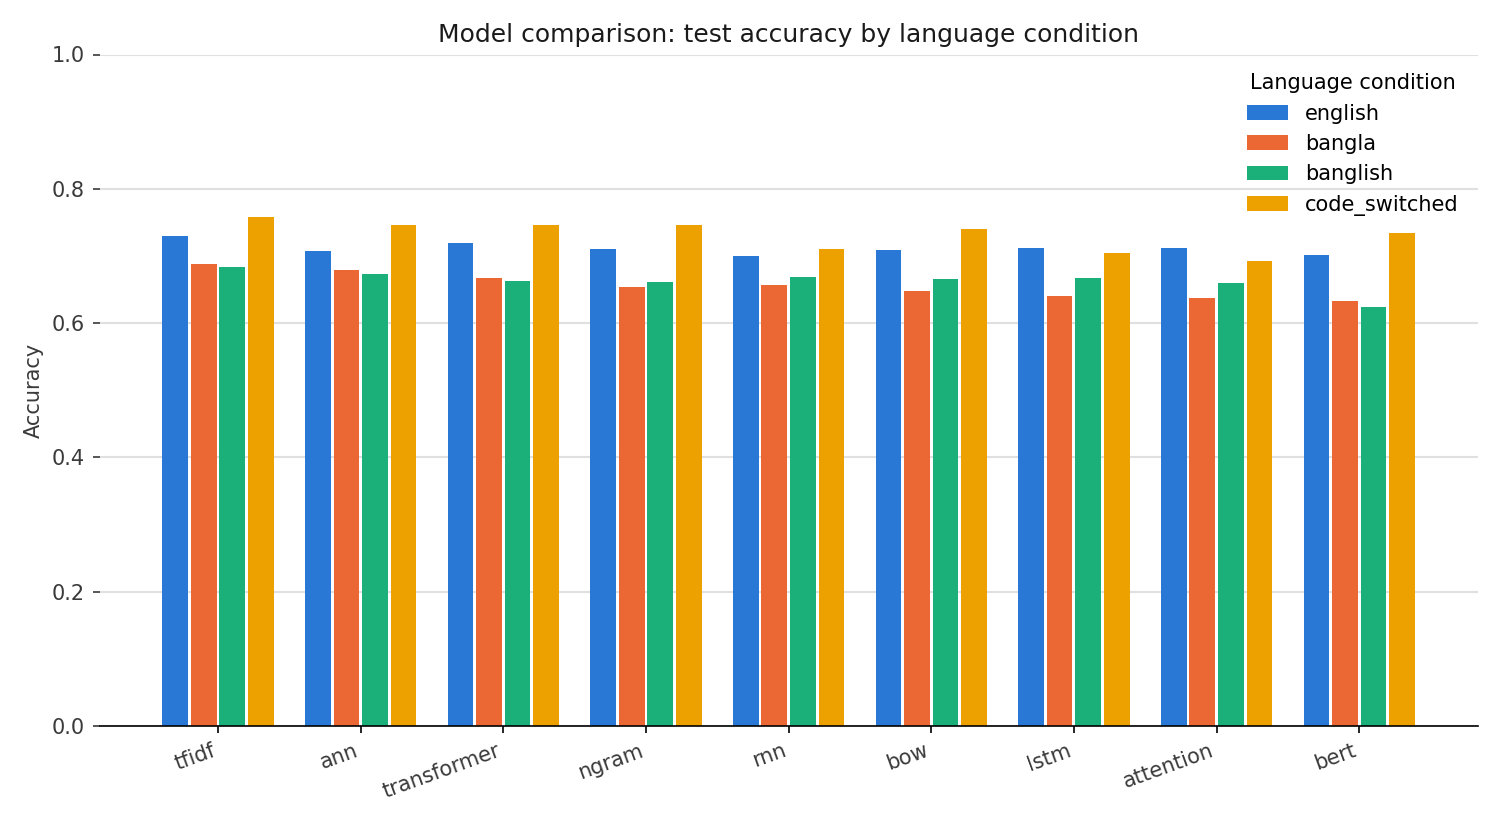
\includegraphics[width=0.95\textwidth]{assets/metrics_comparison.png}
\caption{Test-set accuracy by model and language condition.}
\label{fig:chart}
\end{figure}

TF-IDF with logistic regression is the strongest model on both
cross-validation and the held-out test set, and is the only model to
clear 70\% accuracy. The remaining eight models cluster within a
relatively narrow 65--69\% band; notably, the from-scratch neural models
do not decisively outperform the simplest classical baselines at this
corpus scale, and model rankings shift slightly between the
cross-validation estimate and the single held-out test score (for
example, LSTM ranks second by cross-validation mean but seventh on the
test set) -- a reminder that a single test-set number carries meaningful
sampling variance even at 15{,}000 rows, and that the cross-validated mean
is the more stable estimate of a model's expected performance.

Breaking TF-IDF's result down by language condition (Figure~\ref{fig:chart})
shows accuracy of 72.9\% on English, 68.7\% on Bangla, 68.3\% on Banglish,
and an apparently strong 75.7\% on code-switched text. However, the
code-switched slice contains only 169 test examples, and its macro-F1 is
just 59.8\% -- the \emph{lowest} of the four conditions, versus 73.0\% for
English -- revealing that the high raw accuracy is an artifact of class
imbalance within that small slice rather than genuine robustness. This
pattern held across every model examined, not only TF-IDF.

% =======================================================================
\section{Discussion}
\label{sec:discussion}
% =======================================================================

\textbf{Classical features remain competitive.} At this corpus scale and
with the modest neural hyperparameters used here, TF-IDF's re-weighted
bag-of-phrases representation was not surpassed by any neural
architecture, including the Transformer. This does not imply neural
methods are unsuited to the task -- larger hidden dimensions, more
training epochs, or embeddings pretrained on a larger external corpus
could plausibly close or reverse the gap -- but it is a useful, concrete
reminder that architectural sophistication is not a substitute for
adequate capacity and training budget, and that a strong classical
baseline is worth measuring before assuming a neural model is necessary.

\textbf{Code-switched robustness requires care in measurement.} The
project's central motivating question -- whether these models handle
code-switched input as well as single-script input -- cannot be answered
by accuracy alone when a language condition is this underrepresented.
Macro-F1 corrects for the label imbalance within the code-switched slice
and shows it is, in fact, the hardest condition for every model, matching
the intuitive expectation that intra-sentence language mixing is
genuinely harder to model than single-script text.

\textbf{BERT's result should not be read as ``pretraining did not help.''}
BERT's lower test accuracy is confounded by its much smaller fine-tuning
set (5{,}000 rows versus $\sim$108{,}000) and lower epoch budget, both
deliberate concessions to CPU-only training time. A fairer comparison
would fine-tune BERT on the same data volume as the other models, which
this project's compute budget did not accommodate.

% =======================================================================
\section{Limitations}
% =======================================================================

\begin{itemize}[nosep]
  \item \textbf{Heuristic language labels.} Language-condition tags are
        produced by an automated script-and-dictionary heuristic, not
        human annotation, and inherit that heuristic's edge cases.
  \item \textbf{Code-switched scarcity.} With only 1.1\% of the corpus
        and 169 test examples, conclusions about this condition carry
        wider uncertainty than the other three.
  \item \textbf{Unequal compute budgets.} BERT's smaller fine-tuning
        sample and epoch count (Section~\ref{sec:methodology}) mean its
        result is not a fully controlled comparison against the other
        eight models.
  \item \textbf{Modest neural hyperparameters.} Hidden dimensions, epoch
        counts, and embedding dimensionality were deliberately kept small
        for CPU feasibility; larger budgets may change the ranking.
\end{itemize}

% =======================================================================
\section{Conclusion and Future Work}
% =======================================================================

This project delivered a fully code-driven, 150{,}000-review Bangla--English
code-mixed sentiment corpus and a rigorously cross-validated comparison of
nine sentiment models spanning classical, from-scratch neural, and
pretrained transformer families, packaged with an interactive application
for live exploration. TF-IDF with logistic regression was the strongest
performer overall, and code-switched text was confirmed as the hardest
language condition once evaluated with a class-imbalance-aware metric.
Future work could fine-tune BERT on a training volume comparable to the
other models, collect or synthesize additional code-switched examples
under a clearly documented augmentation policy, and explore larger neural
hyperparameter budgets now that the corpus scale supports them.

\vspace{2em}
\begin{thebibliography}{99}

\bibitem{banglishrev2024}
BanglishRev: A Large-Scale Bangla-English and Code-mixed Dataset of
Product Reviews in E-Commerce. \textit{arXiv preprint arXiv:2412.13161}, 2024.

\bibitem{salton1988term}
G.~Salton and C.~Buckley. Term-weighting approaches in automatic text
retrieval. \textit{Information Processing \& Management}, 24(5):513--523, 1988.

\bibitem{hochreiter1997lstm}
S.~Hochreiter and J.~Schmidhuber. Long short-term memory.
\textit{Neural Computation}, 9(8):1735--1780, 1997.

\bibitem{bahdanau2014attention}
D.~Bahdanau, K.~Cho, and Y.~Bengio. Neural machine translation by jointly
learning to align and translate. \textit{arXiv preprint arXiv:1409.0473}, 2014.

\bibitem{vaswani2017attention}
A.~Vaswani, N.~Shazeer, N.~Parmar, J.~Uszkoreit, L.~Jones, A.~N.~Gomez,
{\L}.~Kaiser, and I.~Polosukhin. Attention is all you need.
\textit{Advances in Neural Information Processing Systems}, 30, 2017.

\bibitem{devlin2019bert}
J.~Devlin, M.-W.~Chang, K.~Lee, and K.~Toutanova. BERT: Pre-training of
deep bidirectional transformers for language understanding.
\textit{Proceedings of NAACL-HLT}, 2019.

\bibitem{pedregosa2011scikit}
F.~Pedregosa et al. Scikit-learn: Machine learning in Python.
\textit{Journal of Machine Learning Research}, 12:2825--2830, 2011.

\end{thebibliography}

\end{document}
